% Generated by Sphinx.
\def\sphinxdocclass{report}
\documentclass[letterpaper,10pt,openany,oneside]{sphinxmanual}
\usepackage[utf8]{inputenc}
\DeclareUnicodeCharacter{00A0}{\nobreakspace}
\usepackage[T1]{fontenc}
\usepackage[english]{babel}
\usepackage{times}
\usepackage[Bjarne]{fncychap}
\usepackage{longtable}
\usepackage{sphinx}
\usepackage{multirow}


\title{Hadoop LastFM Analysis}
\date{August 11, 2014}
\release{}
\author{CSinParallel Project}
\newcommand{\sphinxlogo}{}
\renewcommand{\releasename}{}
\makeindex

\makeatletter
\def\PYG@reset{\let\PYG@it=\relax \let\PYG@bf=\relax%
    \let\PYG@ul=\relax \let\PYG@tc=\relax%
    \let\PYG@bc=\relax \let\PYG@ff=\relax}
\def\PYG@tok#1{\csname PYG@tok@#1\endcsname}
\def\PYG@toks#1+{\ifx\relax#1\empty\else%
    \PYG@tok{#1}\expandafter\PYG@toks\fi}
\def\PYG@do#1{\PYG@bc{\PYG@tc{\PYG@ul{%
    \PYG@it{\PYG@bf{\PYG@ff{#1}}}}}}}
\def\PYG#1#2{\PYG@reset\PYG@toks#1+\relax+\PYG@do{#2}}

\expandafter\def\csname PYG@tok@gd\endcsname{\def\PYG@tc##1{\textcolor[rgb]{0.63,0.00,0.00}{##1}}}
\expandafter\def\csname PYG@tok@gu\endcsname{\let\PYG@bf=\textbf\def\PYG@tc##1{\textcolor[rgb]{0.50,0.00,0.50}{##1}}}
\expandafter\def\csname PYG@tok@gt\endcsname{\def\PYG@tc##1{\textcolor[rgb]{0.00,0.25,0.82}{##1}}}
\expandafter\def\csname PYG@tok@gs\endcsname{\let\PYG@bf=\textbf}
\expandafter\def\csname PYG@tok@gr\endcsname{\def\PYG@tc##1{\textcolor[rgb]{1.00,0.00,0.00}{##1}}}
\expandafter\def\csname PYG@tok@cm\endcsname{\let\PYG@it=\textit\def\PYG@tc##1{\textcolor[rgb]{0.25,0.50,0.56}{##1}}}
\expandafter\def\csname PYG@tok@vg\endcsname{\def\PYG@tc##1{\textcolor[rgb]{0.73,0.38,0.84}{##1}}}
\expandafter\def\csname PYG@tok@m\endcsname{\def\PYG@tc##1{\textcolor[rgb]{0.13,0.50,0.31}{##1}}}
\expandafter\def\csname PYG@tok@mh\endcsname{\def\PYG@tc##1{\textcolor[rgb]{0.13,0.50,0.31}{##1}}}
\expandafter\def\csname PYG@tok@cs\endcsname{\def\PYG@tc##1{\textcolor[rgb]{0.25,0.50,0.56}{##1}}\def\PYG@bc##1{\setlength{\fboxsep}{0pt}\colorbox[rgb]{1.00,0.94,0.94}{\strut ##1}}}
\expandafter\def\csname PYG@tok@ge\endcsname{\let\PYG@it=\textit}
\expandafter\def\csname PYG@tok@vc\endcsname{\def\PYG@tc##1{\textcolor[rgb]{0.73,0.38,0.84}{##1}}}
\expandafter\def\csname PYG@tok@il\endcsname{\def\PYG@tc##1{\textcolor[rgb]{0.13,0.50,0.31}{##1}}}
\expandafter\def\csname PYG@tok@go\endcsname{\def\PYG@tc##1{\textcolor[rgb]{0.19,0.19,0.19}{##1}}}
\expandafter\def\csname PYG@tok@cp\endcsname{\def\PYG@tc##1{\textcolor[rgb]{0.00,0.44,0.13}{##1}}}
\expandafter\def\csname PYG@tok@gi\endcsname{\def\PYG@tc##1{\textcolor[rgb]{0.00,0.63,0.00}{##1}}}
\expandafter\def\csname PYG@tok@gh\endcsname{\let\PYG@bf=\textbf\def\PYG@tc##1{\textcolor[rgb]{0.00,0.00,0.50}{##1}}}
\expandafter\def\csname PYG@tok@ni\endcsname{\let\PYG@bf=\textbf\def\PYG@tc##1{\textcolor[rgb]{0.84,0.33,0.22}{##1}}}
\expandafter\def\csname PYG@tok@nl\endcsname{\let\PYG@bf=\textbf\def\PYG@tc##1{\textcolor[rgb]{0.00,0.13,0.44}{##1}}}
\expandafter\def\csname PYG@tok@nn\endcsname{\let\PYG@bf=\textbf\def\PYG@tc##1{\textcolor[rgb]{0.05,0.52,0.71}{##1}}}
\expandafter\def\csname PYG@tok@no\endcsname{\def\PYG@tc##1{\textcolor[rgb]{0.38,0.68,0.84}{##1}}}
\expandafter\def\csname PYG@tok@na\endcsname{\def\PYG@tc##1{\textcolor[rgb]{0.25,0.44,0.63}{##1}}}
\expandafter\def\csname PYG@tok@nb\endcsname{\def\PYG@tc##1{\textcolor[rgb]{0.00,0.44,0.13}{##1}}}
\expandafter\def\csname PYG@tok@nc\endcsname{\let\PYG@bf=\textbf\def\PYG@tc##1{\textcolor[rgb]{0.05,0.52,0.71}{##1}}}
\expandafter\def\csname PYG@tok@nd\endcsname{\let\PYG@bf=\textbf\def\PYG@tc##1{\textcolor[rgb]{0.33,0.33,0.33}{##1}}}
\expandafter\def\csname PYG@tok@ne\endcsname{\def\PYG@tc##1{\textcolor[rgb]{0.00,0.44,0.13}{##1}}}
\expandafter\def\csname PYG@tok@nf\endcsname{\def\PYG@tc##1{\textcolor[rgb]{0.02,0.16,0.49}{##1}}}
\expandafter\def\csname PYG@tok@si\endcsname{\let\PYG@it=\textit\def\PYG@tc##1{\textcolor[rgb]{0.44,0.63,0.82}{##1}}}
\expandafter\def\csname PYG@tok@s2\endcsname{\def\PYG@tc##1{\textcolor[rgb]{0.25,0.44,0.63}{##1}}}
\expandafter\def\csname PYG@tok@vi\endcsname{\def\PYG@tc##1{\textcolor[rgb]{0.73,0.38,0.84}{##1}}}
\expandafter\def\csname PYG@tok@nt\endcsname{\let\PYG@bf=\textbf\def\PYG@tc##1{\textcolor[rgb]{0.02,0.16,0.45}{##1}}}
\expandafter\def\csname PYG@tok@nv\endcsname{\def\PYG@tc##1{\textcolor[rgb]{0.73,0.38,0.84}{##1}}}
\expandafter\def\csname PYG@tok@s1\endcsname{\def\PYG@tc##1{\textcolor[rgb]{0.25,0.44,0.63}{##1}}}
\expandafter\def\csname PYG@tok@gp\endcsname{\let\PYG@bf=\textbf\def\PYG@tc##1{\textcolor[rgb]{0.78,0.36,0.04}{##1}}}
\expandafter\def\csname PYG@tok@sh\endcsname{\def\PYG@tc##1{\textcolor[rgb]{0.25,0.44,0.63}{##1}}}
\expandafter\def\csname PYG@tok@ow\endcsname{\let\PYG@bf=\textbf\def\PYG@tc##1{\textcolor[rgb]{0.00,0.44,0.13}{##1}}}
\expandafter\def\csname PYG@tok@sx\endcsname{\def\PYG@tc##1{\textcolor[rgb]{0.78,0.36,0.04}{##1}}}
\expandafter\def\csname PYG@tok@bp\endcsname{\def\PYG@tc##1{\textcolor[rgb]{0.00,0.44,0.13}{##1}}}
\expandafter\def\csname PYG@tok@c1\endcsname{\let\PYG@it=\textit\def\PYG@tc##1{\textcolor[rgb]{0.25,0.50,0.56}{##1}}}
\expandafter\def\csname PYG@tok@kc\endcsname{\let\PYG@bf=\textbf\def\PYG@tc##1{\textcolor[rgb]{0.00,0.44,0.13}{##1}}}
\expandafter\def\csname PYG@tok@c\endcsname{\let\PYG@it=\textit\def\PYG@tc##1{\textcolor[rgb]{0.25,0.50,0.56}{##1}}}
\expandafter\def\csname PYG@tok@mf\endcsname{\def\PYG@tc##1{\textcolor[rgb]{0.13,0.50,0.31}{##1}}}
\expandafter\def\csname PYG@tok@err\endcsname{\def\PYG@bc##1{\setlength{\fboxsep}{0pt}\fcolorbox[rgb]{1.00,0.00,0.00}{1,1,1}{\strut ##1}}}
\expandafter\def\csname PYG@tok@kd\endcsname{\let\PYG@bf=\textbf\def\PYG@tc##1{\textcolor[rgb]{0.00,0.44,0.13}{##1}}}
\expandafter\def\csname PYG@tok@ss\endcsname{\def\PYG@tc##1{\textcolor[rgb]{0.32,0.47,0.09}{##1}}}
\expandafter\def\csname PYG@tok@sr\endcsname{\def\PYG@tc##1{\textcolor[rgb]{0.14,0.33,0.53}{##1}}}
\expandafter\def\csname PYG@tok@mo\endcsname{\def\PYG@tc##1{\textcolor[rgb]{0.13,0.50,0.31}{##1}}}
\expandafter\def\csname PYG@tok@mi\endcsname{\def\PYG@tc##1{\textcolor[rgb]{0.13,0.50,0.31}{##1}}}
\expandafter\def\csname PYG@tok@kn\endcsname{\let\PYG@bf=\textbf\def\PYG@tc##1{\textcolor[rgb]{0.00,0.44,0.13}{##1}}}
\expandafter\def\csname PYG@tok@o\endcsname{\def\PYG@tc##1{\textcolor[rgb]{0.40,0.40,0.40}{##1}}}
\expandafter\def\csname PYG@tok@kr\endcsname{\let\PYG@bf=\textbf\def\PYG@tc##1{\textcolor[rgb]{0.00,0.44,0.13}{##1}}}
\expandafter\def\csname PYG@tok@s\endcsname{\def\PYG@tc##1{\textcolor[rgb]{0.25,0.44,0.63}{##1}}}
\expandafter\def\csname PYG@tok@kp\endcsname{\def\PYG@tc##1{\textcolor[rgb]{0.00,0.44,0.13}{##1}}}
\expandafter\def\csname PYG@tok@w\endcsname{\def\PYG@tc##1{\textcolor[rgb]{0.73,0.73,0.73}{##1}}}
\expandafter\def\csname PYG@tok@kt\endcsname{\def\PYG@tc##1{\textcolor[rgb]{0.56,0.13,0.00}{##1}}}
\expandafter\def\csname PYG@tok@sc\endcsname{\def\PYG@tc##1{\textcolor[rgb]{0.25,0.44,0.63}{##1}}}
\expandafter\def\csname PYG@tok@sb\endcsname{\def\PYG@tc##1{\textcolor[rgb]{0.25,0.44,0.63}{##1}}}
\expandafter\def\csname PYG@tok@k\endcsname{\let\PYG@bf=\textbf\def\PYG@tc##1{\textcolor[rgb]{0.00,0.44,0.13}{##1}}}
\expandafter\def\csname PYG@tok@se\endcsname{\let\PYG@bf=\textbf\def\PYG@tc##1{\textcolor[rgb]{0.25,0.44,0.63}{##1}}}
\expandafter\def\csname PYG@tok@sd\endcsname{\let\PYG@it=\textit\def\PYG@tc##1{\textcolor[rgb]{0.25,0.44,0.63}{##1}}}

\def\PYGZbs{\char`\\}
\def\PYGZus{\char`\_}
\def\PYGZob{\char`\{}
\def\PYGZcb{\char`\}}
\def\PYGZca{\char`\^}
\def\PYGZam{\char`\&}
\def\PYGZlt{\char`\<}
\def\PYGZgt{\char`\>}
\def\PYGZsh{\char`\#}
\def\PYGZpc{\char`\%}
\def\PYGZdl{\char`\$}
\def\PYGZti{\char`\~}
% for compatibility with earlier versions
\def\PYGZat{@}
\def\PYGZlb{[}
\def\PYGZrb{]}
\makeatother

\begin{document}

\maketitle
\tableofcontents
\phantomsection\label{index::doc}


This module demonstrates how hadoop and WMR can be used to
analize the lastFM million song dataset. It encorporates several
advanced hadoop techniques such as job chaining and multiple
input. Students should know how to use the WMR hadoop interface
before beginning this module.

The dataset was obtained from Columbia University's
\href{http://labrosa.ee.columbia.edu/millionsong/lastfm}{LabROSA}.
However it has been converted into a format that is easier to work
with on WMR. The edited dataset is also much smaller since it doesn't
include the audio analysis information. If you would like the smaller
dataset for your own WMR cluster please contact \href{mailto:JLyman@macalester.edu}{JLyman@macalester.edu}


\chapter{The Million Song Dataset}
\label{0-Introduction/Introduction::doc}\label{0-Introduction/Introduction:the-million-song-dataset}\label{0-Introduction/Introduction:hadoop-lastfm-analysis}
Last.fm is a popular music recommendation website that tracks
what it's users listen to and then suggests similar songs.
It provides an API which can be used to retrieve metadata about
specific songs.

Researchers at Columbia's LabROSA used this api to generate a
dataset containing 1,000,000 songs from 44,745 artists. For our
purposes this data has been split into 3 different tab separated
files.

Each file has a different prefix which hadoop passes to the
mapper as a key. The rest of the data is passed to the mapper as
the value. Each file contains several fields so it is necessary
to call value.split(`t') to access them.
\setbox0\vbox{
\begin{minipage}{0.95\linewidth}
\textbf{System-dependent Alert}

\medskip


The path of each of the datasets shown below may not be the same on your WMR system.
It is correct for this WMR server:

selkie.macalester.edu/wmr
\end{minipage}}
\begin{center}\setlength{\fboxsep}{5pt}\shadowbox{\box0}\end{center}
\begin{itemize}
\item {} 
\textbf{/shared/lastfm/similars.tsv} contains information about artists
who are similar to each other. The prefix used to tag each group
of artists is ``similar'' (the key for the mapper). The
first value of the data after that tag is the id of an artist and the rest
of the values are the ids of similar artists. The list of
similar artists varies in size. If artist A's list contains B
and C there is no guarantee that B's list contains C or A.
The list of similar artists varies in length and may be empty.

Here is what a small portion of the first line of this file looks like:

\begin{Verbatim}[commandchars=\\\{\}]
similar     ARRPV2V1187B9B6312      ARDDLVP1187B98CB8A      AR3M0PY119B86695E3      ARC1X4C1187B98CF3A
\end{Verbatim}

\item {} 
\textbf{/shared/lastfm/terms.tsv} contains musical terms associated with artists.
The prefix beginning each line is ``term'' (the key for the mapper). The first
value of the data is an artist id and the rest of the values
are comma separated triplets representing terms associated
with the artist. They can be separated by calling
term.split(`,')
\begin{itemize}
\item {} 
The first value is the term itself. It may be a genres like
``rock'' or ``pop'' or a descriptor like ``london''

\item {} 
The second value is the frequency with which that term is
used in reference to the artist, it is a float from 0-1

\item {} 
The last value is the weight of the term which provides a
a measure of how well a given term is to describes the
an artist. For example `rock' is frequently used to
describe the Beatles, but ``british invasion'' is more
descriptive so it has a higher weight. The weight is a
float from 0-1

\end{itemize}

there are a variable number of terms associated with each
artist and there may be none.
Here is a small portion of the first line of this file:

\begin{Verbatim}[commandchars=\\\{\}]
term        ARRPV2V1187B9B6312      hard house,0.934636697674,1.0   viking metal,0.849886186054,0.93429655287       jam band,0.849886186054,0.93429655287
\end{Verbatim}

\item {} 
\textbf{/shared/lastfm/metadata.tsv} is prefixed with ``metadata''.
The data contains 25 different fields of metadata about a given
song, which are explained in the following chart. These fields may be null (for strings)
on nan (not a number, for floats).

\end{itemize}

\begin{tabulary}{\linewidth}{|L|L|L|}
\hline
\textbf{
index
} & \textbf{
value
} & \textbf{
Description
}\\\hline

0
 & 
track id
 & 
String
\\\hline

1
 & 
title
 & 
String
\\\hline

2
 & 
release name (album)
 & 
String
\\\hline

3
 & 
year
 & 
Int
\\\hline

4
 & 
artist name
 & 
String
\\\hline

5
 & 
artist id
 & 
String
\\\hline

6
 & 
artist familiarity
 & 
Float 0-1 How well known an artist is
\\\hline

7
 & 
artist hotness
 & 
Float 0-1 Current popularity of an artist
\\\hline

8
 & 
artist latitude
 & 
Float
\\\hline

9
 & 
artist longitude
 & 
Float
\\\hline

10
 & 
artist location
 & 
String
\\\hline

11
 & 
hotness
 & 
Float 0-1 current popularity of a song
\\\hline

12
 & 
danceablity
 & 
Float 0-1
\\\hline

13
 & 
duration
 & 
Float number of seconds in a song
\\\hline

14
 & 
energy
 & 
Float 0-1
\\\hline

15
 & 
loudness
 & 
Float 0-1
\\\hline

16
 & 
end of fade in
 & 
Float
\\\hline

17
 & 
start of fade out
 & 
Float
\\\hline

18
 & 
tempo
 & 
Float tempo in beats per minute
\\\hline

19
 & 
time signature
 & 
Int number of beats per measure
\\\hline

20
 & 
time signature confidence
 & 
Float 0-1 confidence in the above number
\\\hline

21
 & 
mode
 & 
1 for major 0 for minor
\\\hline

22
 & 
mode confidence
 & 
Float 0-1 confidence in the above number
\\\hline

23
 & 
key
 & 
Int C=0, C\#=1, D=2...
\\\hline

24
 & 
key confidence
 & 
Float 0-1 confidence in the above number
\\\hline
\end{tabulary}


Here is the first line of this file (intentionally wrapped so you can see all the values;
it contains no newlines except for the ending one it the real file):

\begin{Verbatim}[commandchars=\\\{\}]
metadata    TRAMMDT128F934E8C5      Wicked City     Stuntrock (Original Soundtrack) 0
Sorcery     ARRPV2V1187B9B6312      0.433976792653  0.335432931443  40.82559        -74.10874
null        nan     0.0     257.14893       0.0     -10.068 0.195   253.063 122.771 4       0.812
0   0.439   4       0.383
\end{Verbatim}

\begin{notice}{note}{Note:}
The year in the above line of data, the third element counting from 0 after the ``metadata''
tag prefix, is given as 0.
\end{notice}


\chapter{Fun with key signatures}
\label{1-Keys/Keys:fun-with-key-signatures}\label{1-Keys/Keys::doc}
Let's get our hands dirty by answering a practice question:
What is the most common key signature in the dataset?

A key signature is made up by a key (C, G\#, etc) and a mode,
either major or minor (these aren't the only modes, but they are
the only ones in the dataset). Both the key and the mode are
important, because A minor and C major contain the same notes so
if our mode is incorrect we will get bad results.

Luckily the dataset provides us with a measure of how accurate
it's guesses for the key and the mode are. These are both floats
from 0-1 so to find the confidence in the key signature we'll
multiply them, that way if the key is certain but the mode is
totally unknown, the confidence will be low.


\section{Coding the Hadoop Job}
\label{1-Keys/Keys:coding-the-hadoop-job}
A glance at the chart from last chapter tells us that the key and
key confidence are stored at indices 23 and 24 respectively and
that the mode and mode confidence are stored at indices 21 and 22
respectively.

Armed with this information we can write a mapper that emits a
key signature as a key and the confidence as a value.
We'll also perform a basic sanity check on our data by testing to
see if all 25 feilds are present. It's good practice to sanity
check data in the mapper because you can never be certain that
your data is pure.

Our \code{mapper} looks like this:

\begin{Verbatim}[commandchars=\\\{\},numbers=left,firstnumber=1,stepnumber=1]
\PYG{k}{def} \PYG{n+nf}{mapper}\PYG{p}{(}\PYG{n}{key}\PYG{p}{,} \PYG{n}{value}\PYG{p}{)}\PYG{p}{:}
  \PYG{n}{data} \PYG{o}{=} \PYG{n}{value}\PYG{o}{.}\PYG{n}{split}\PYG{p}{(}\PYG{l+s}{'}\PYG{l+s+se}{\PYGZbs{}t}\PYG{l+s}{'}\PYG{p}{)}
  \PYG{k}{if} \PYG{n+nb}{len}\PYG{p}{(}\PYG{n}{data}\PYG{p}{)} \PYG{o}{==} \PYG{l+m+mi}{25}\PYG{p}{:}
    \PYG{n}{keySig} \PYG{o}{=} \PYG{p}{(}\PYG{n}{data}\PYG{p}{[}\PYG{l+m+mi}{23}\PYG{p}{]}\PYG{p}{,} \PYG{n}{data}\PYG{p}{[}\PYG{l+m+mi}{21}\PYG{p}{]}\PYG{p}{)}
    \PYG{n}{confidence} \PYG{o}{=} \PYG{n+nb}{float}\PYG{p}{(}\PYG{n}{data}\PYG{p}{[}\PYG{l+m+mi}{24}\PYG{p}{]}\PYG{p}{)} \PYG{o}{*} \PYG{n+nb}{float}\PYG{p}{(}\PYG{n}{data}\PYG{p}{[}\PYG{l+m+mi}{22}\PYG{p}{]}\PYG{p}{)}
    \PYG{n}{Wmr}\PYG{o}{.}\PYG{n}{emit}\PYG{p}{(}\PYG{n}{keySig}\PYG{p}{,} \PYG{n}{confidence}\PYG{p}{)}
\end{Verbatim}

\begin{notice}{note}{Note:}
Remember, WMR interprets all keys and values as strings,
however we're using a tuple as a key and a float as a
value. This is okay since they get automatically cast by
WMR, we just have to remember to recast them in the
reducer. Python's eval() method is useful for getting tuples
from strings
\end{notice}

Our \code{reducer} will sum up all of the confidences. This way songs
that have higher confidences will have more influence on the
total than songs with uncertain keys. It also turns the key
signatures from numbers into something more human readable. Doing
the conversion in the reducer instead of the mapper saves a lot
of work because, the calculation is only performed once per each
of the 24 keys rather than once per each of the million songs

\begin{Verbatim}[commandchars=\\\{\},numbers=left,firstnumber=1,stepnumber=1]
\PYG{k}{def} \PYG{n+nf}{reducer}\PYG{p}{(}\PYG{n}{key}\PYG{p}{,} \PYG{n}{values}\PYG{p}{)}\PYG{p}{:}
  \PYG{n}{keys} \PYG{o}{=} \PYG{p}{[}\PYG{l+s}{'}\PYG{l+s}{C}\PYG{l+s}{'}\PYG{p}{,}\PYG{l+s}{'}\PYG{l+s}{C\PYGZsh{}}\PYG{l+s}{'}\PYG{p}{,}\PYG{l+s}{'}\PYG{l+s}{D}\PYG{l+s}{'}\PYG{p}{,}\PYG{l+s}{'}\PYG{l+s}{D\PYGZsh{}}\PYG{l+s}{'}\PYG{p}{,}\PYG{l+s}{'}\PYG{l+s}{E}\PYG{l+s}{'}\PYG{p}{,}\PYG{l+s}{'}\PYG{l+s}{F}\PYG{l+s}{'}\PYG{p}{,}\PYG{l+s}{'}\PYG{l+s}{F\PYGZsh{}}\PYG{l+s}{'}\PYG{p}{,}\PYG{l+s}{'}\PYG{l+s}{G}\PYG{l+s}{'}\PYG{p}{,}\PYG{l+s}{'}\PYG{l+s}{G\PYGZsh{}}\PYG{l+s}{'}\PYG{p}{,}\PYG{l+s}{'}\PYG{l+s}{A}\PYG{l+s}{'}\PYG{p}{,}\PYG{l+s}{'}\PYG{l+s}{A\PYGZsh{}}\PYG{l+s}{'}\PYG{p}{,}\PYG{l+s}{'}\PYG{l+s}{B}\PYG{l+s}{'}\PYG{p}{]}
  \PYG{n}{keySig}\PYG{p}{,} \PYG{n}{mode} \PYG{o}{=} \PYG{n+nb}{eval}\PYG{p}{(}\PYG{n}{key}\PYG{p}{)}
  \PYG{n}{keySig} \PYG{o}{=} \PYG{n}{keys}\PYG{p}{[}\PYG{n+nb}{int}\PYG{p}{(}\PYG{n}{keySig}\PYG{p}{)}\PYG{p}{]}
  \PYG{k}{if} \PYG{n}{mode} \PYG{o}{==} \PYG{l+s}{'}\PYG{l+s}{0}\PYG{l+s}{'}\PYG{p}{:}
    \PYG{n}{keySig} \PYG{o}{+}\PYG{o}{=} \PYG{l+s}{'}\PYG{l+s}{m}\PYG{l+s}{'}
  \PYG{n}{count} \PYG{o}{=} \PYG{l+m+mf}{0.0}
  \PYG{k}{for} \PYG{n}{value} \PYG{o+ow}{in} \PYG{n}{values}\PYG{p}{:}
    \PYG{n}{count} \PYG{o}{+}\PYG{o}{=} \PYG{n+nb}{float}\PYG{p}{(}\PYG{n}{value}\PYG{p}{)}
  \PYG{n}{Wmr}\PYG{o}{.}\PYG{n}{emit}\PYG{p}{(}\PYG{n}{key}\PYG{p}{,} \PYG{n}{count}\PYG{p}{)}
\end{Verbatim}

After running the job we find that the most common key is G major
and the least common is D\#/E flat minor.


\section{Going Further}
\label{1-Keys/Keys:going-further}
Why is G the most popular key? One reason could be the guitar.
The fingerings for chords in the key of G are all very simple so
maybe artists pick to G because it's easy. If this theory is
true, then genres like rock and country that use more guitars
should use the key of G more often than genres like
Hip Hop and electronic.

Unfortunately our dataset only has artist level tags, so we will
need to create a filtering job that only outputs songs by artists
who have been tagged with a specific genre.

This means that our hadoop job will have to read input from
both the terms file and the metadata file. We can do this by
using /shared/lastfm/ as the input path. Since it is a folder,
all of the files in the folder are used as input. We want to pull
different peices of information from each of these files
\begin{itemize}
\item {} 
\textbf{From metadata:} the key signature and confidence of a song

\item {} 
\textbf{From terms:} whether the genre is in the terms list and has
a weight greater than 0.5

\end{itemize}

We want to send all of this information to the reducers
sorted by artist. The artist ID of a song is at index 5 of the
metadata file and the artist ID is at index 0 in the terms file.
We can let the reducer know what information is being passed to
it by emiting tuples where the first value is a flag stating what
the second value is.

With this information we can write a \code{mapper (genreMapper.py).}.
Remember to perform
the sanity check on the metadata. Unfortuneately we can't run
the same check on the other files because they have variable
line lengths.

\begin{Verbatim}[commandchars=\\\{\},numbers=left,firstnumber=1,stepnumber=1]
\PYG{k}{def} \PYG{n+nf}{mapper}\PYG{p}{(}\PYG{n}{key}\PYG{p}{,} \PYG{n}{value}\PYG{p}{)}\PYG{p}{:}
  \PYG{n}{genre} \PYG{o}{=} \PYG{l+s}{"}\PYG{l+s}{rock}\PYG{l+s}{"}
  \PYG{n}{data} \PYG{o}{=} \PYG{n}{value}\PYG{o}{.}\PYG{n}{split}\PYG{p}{(}\PYG{l+s}{'}\PYG{l+s+se}{\PYGZbs{}t}\PYG{l+s}{'}\PYG{p}{)}
  \PYG{k}{if} \PYG{n}{key} \PYG{o}{==} \PYG{l+s}{"}\PYG{l+s}{metadata}\PYG{l+s}{"} \PYG{o+ow}{and} \PYG{n+nb}{len}\PYG{p}{(}\PYG{n}{data}\PYG{p}{)} \PYG{o}{==} \PYG{l+m+mi}{25}\PYG{p}{:}
    \PYG{n}{artist} \PYG{o}{=} \PYG{n}{data}\PYG{p}{[}\PYG{l+m+mi}{5}\PYG{p}{]}
    \PYG{n}{keySig} \PYG{o}{=} \PYG{p}{(}\PYG{n}{data}\PYG{p}{[}\PYG{l+m+mi}{23}\PYG{p}{]}\PYG{p}{,} \PYG{n}{data}\PYG{p}{[}\PYG{l+m+mi}{21}\PYG{p}{]}\PYG{p}{)}
    \PYG{n}{confidence} \PYG{o}{=} \PYG{n+nb}{float}\PYG{p}{(}\PYG{n}{data}\PYG{p}{[}\PYG{l+m+mi}{24}\PYG{p}{]}\PYG{p}{)} \PYG{o}{*} \PYG{n+nb}{float}\PYG{p}{(}\PYG{n}{data}\PYG{p}{[}\PYG{l+m+mi}{22}\PYG{p}{]}\PYG{p}{)}
    \PYG{n}{Wmr}\PYG{o}{.}\PYG{n}{emit}\PYG{p}{(}\PYG{n}{artist}\PYG{p}{,} \PYG{p}{(}\PYG{l+s}{"}\PYG{l+s}{song}\PYG{l+s}{"}\PYG{p}{,} \PYG{p}{(}\PYG{n}{keySig}\PYG{p}{,} \PYG{n}{confidence}\PYG{p}{)}\PYG{p}{)}\PYG{p}{)}
  \PYG{k}{elif} \PYG{n}{key} \PYG{o}{==} \PYG{l+s}{"}\PYG{l+s}{term}\PYG{l+s}{"}\PYG{p}{:}
    \PYG{n}{artist} \PYG{o}{=} \PYG{n}{data}\PYG{p}{[}\PYG{l+m+mi}{0}\PYG{p}{]}
    \PYG{k}{for} \PYG{n}{triplet} \PYG{o+ow}{in} \PYG{n}{data}\PYG{p}{[}\PYG{l+m+mi}{1}\PYG{p}{:}\PYG{p}{]}\PYG{p}{:}
      \PYG{n}{term}\PYG{p}{,} \PYG{n}{freq}\PYG{p}{,} \PYG{n}{weight} \PYG{o}{=} \PYG{n}{triplet}\PYG{o}{.}\PYG{n}{split}\PYG{p}{(}\PYG{l+s}{'}\PYG{l+s}{,}\PYG{l+s}{'}\PYG{p}{)}
      \PYG{k}{if} \PYG{n}{term} \PYG{o}{==} \PYG{n}{genre} \PYG{o+ow}{and} \PYG{n+nb}{float}\PYG{p}{(}\PYG{n}{weight}\PYG{p}{)} \PYG{o}{\PYGZgt{}} \PYG{l+m+mf}{0.5}\PYG{p}{:}
        \PYG{n}{Wmr}\PYG{o}{.}\PYG{n}{emit}\PYG{p}{(}\PYG{n}{artist}\PYG{p}{,} \PYG{p}{(}\PYG{l+s}{"}\PYG{l+s}{term}\PYG{l+s}{"}\PYG{p}{,} \PYG{n+nb+bp}{True}\PYG{p}{)}\PYG{p}{)}
\end{Verbatim}

Our \code{reducer (genreReducer.py)} will need to take all of this data and only emit
the songs by artists who are tagged with the the genre.

\begin{Verbatim}[commandchars=\\\{\},numbers=left,firstnumber=1,stepnumber=1]
\PYG{k}{def} \PYG{n+nf}{reducer}\PYG{p}{(}\PYG{n}{key}\PYG{p}{,} \PYG{n}{values}\PYG{p}{)}\PYG{p}{:}
  \PYG{n}{isMatch} \PYG{o}{=} \PYG{n+nb+bp}{False}
  \PYG{n}{songPairs} \PYG{o}{=} \PYG{p}{[}\PYG{p}{]}
  \PYG{k}{for} \PYG{n}{value} \PYG{o+ow}{in} \PYG{n}{values}\PYG{p}{:}
    \PYG{n}{flag}\PYG{p}{,} \PYG{n}{data} \PYG{o}{=} \PYG{n+nb}{eval}\PYG{p}{(}\PYG{n}{value}\PYG{p}{)}
    \PYG{k}{if} \PYG{n}{flag} \PYG{o}{==} \PYG{l+s}{"}\PYG{l+s}{term}\PYG{l+s}{"}\PYG{p}{:}
      \PYG{n}{isMatch} \PYG{o}{=} \PYG{n}{data}
    \PYG{k}{elif} \PYG{n}{flag} \PYG{o}{==} \PYG{l+s}{"}\PYG{l+s}{song}\PYG{l+s}{"}\PYG{p}{:}
      \PYG{n}{songPairs}\PYG{o}{.}\PYG{n}{append}\PYG{p}{(}\PYG{n}{data}\PYG{p}{)}
  \PYG{k}{if} \PYG{n}{isMatch}\PYG{p}{:}
    \PYG{k}{for} \PYG{n}{keySig}\PYG{p}{,} \PYG{n}{confidence} \PYG{o+ow}{in} \PYG{n}{songPairs}\PYG{p}{:}
      \PYG{n}{Wmr}\PYG{o}{.}\PYG{n}{emit}\PYG{p}{(}\PYG{n}{keySig}\PYG{p}{,} \PYG{n}{confidence}\PYG{p}{)}
\end{Verbatim}

After running this job we are left with a list of key signatures
and confidences. We still need to add up the confidences for each
of the key signatures. We can do this by passing our list to the
\code{reducer (avgKeyReducer.py)}
from the first part of this module. To use the output of
a Wmr job as input for another, just click the `Use Output' on
either the top or the bottom of the page.

To pass our data straight to the reducer we'll use what's known
as the \code{identity mapper}:

\begin{Verbatim}[commandchars=\\\{\},numbers=left,firstnumber=1,stepnumber=1]
\PYG{k}{def} \PYG{n+nf}{mapper}\PYG{p}{(}\PYG{n}{key}\PYG{p}{,} \PYG{n}{value}\PYG{p}{)}\PYG{p}{:}
  \PYG{n}{Wmr}\PYG{o}{.}\PYG{n}{emit}\PYG{p}{(}\PYG{n}{key}\PYG{p}{,} \PYG{n}{value}\PYG{p}{)}
\end{Verbatim}

Try running this compound job for different values of genre. All
of the tags in the terms file are lowercase. Once you've finished
make a graph of the percentage of songs that are in each key per
genre. It should look something like this:

{\hfill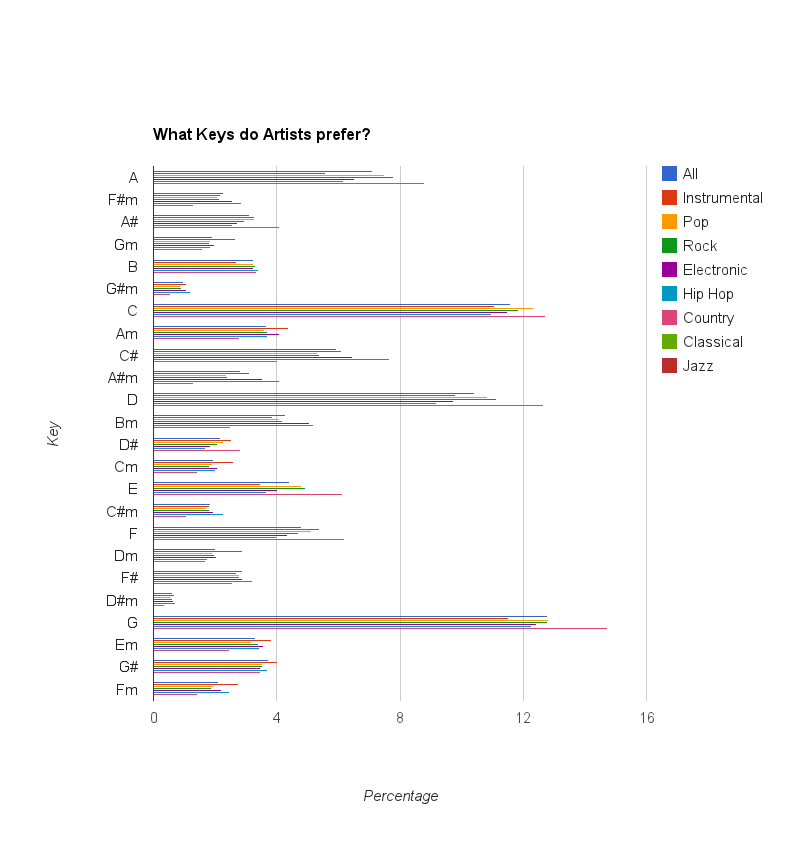
\includegraphics{keyChart.png}\hfill}


\section{Interpretting the results}
\label{1-Keys/Keys:interpretting-the-results}
It looks like G is the most popular key for every genre but
classical where it barely looses out to C. In country music G
is a heavy favorite along with C and D which are also relatively
easy keys to play on the guitar. However G is also very popular
in electronic and hip hop, genres where the voice is often the
only acoustic instrument.

Overall it seems like the guitar does have some effect on an
artist's choice of key, but it can't be explained by guitar
tuning alone.


\section{Challenge}
\label{1-Keys/Keys:challenge}
Can you find a way to find the counts for 6 different genres using only
one chain of jobs?


\chapter{Challenge Problems}
\label{2-Challenges/Challenges:challenge-problems}\label{2-Challenges/Challenges::doc}
Now that you're familiar with the dataset try some of these
challenge problems. Be careful, some songs are missing fields
\begin{itemize}
\item {} 
Find the average artist familiarity. This information is stored
in the metadata file at index 6 so you'll have to find a way
to make sure that each artist is only counted once

\item {} 
Find the average danceablity of an artist's songs. Compare it
with the artist's familiarity. Is there a correlation between
them?

\item {} 
Find the duration of the fade in/out for each song. Plot your
results by year. How have tastes changed over time?

\item {} 
Do similar artists have similar danceabilities, energies, and
loudnesses?

\end{itemize}



\renewcommand{\indexname}{Index}
\printindex
\end{document}
